\section{Description of the Experiment}
  \label{sec:twophoton_experiment}

    The experimental work in this chapter was carried out by Lee Weller, and a
    full description may be found in Weller, 2013\cite{Weller2013a}.

    A high-intensity \textsc{cw} laser beam, near-resonant with the \textsc{d2}
    lines, was incident on a thermal vapour cell of rubidium atoms in their
    natural isotopic abundances. The \textsc{d2} lines represent resonant
    transitions from the $5^2\rm{S}_{\nicefrac{1}{2}}$ ground state of the
    atom to the $5^2\rm{P}_{\nicefrac{3}{2}}$ excited state manifold. The
    Pyrex cell had a length of \unit[$2$]{mm} in the propagation direction $z$
    and sat in a thermal oven. The beam had a waist (\ie $\nicefrac{1}{e^2}$
    radius) of \unit[$6.6\pm0.2$]{$\mu$m} and a power of \unit[$80$]{mW},
    providing a peak beam intensity of 
    \unit[$1.2\times10^5$]{W~cm$^{-2}$}\cite{Weller2013a}.

    A lens was used to image fluorescence onto a multi-mode fibre connected to a
    spectrometer. This revealed fluorescence from excited states that cannot be
    accessed energetically from individual photon excitations near-resonant with
    the \textsc{d2} transitions. In order to investigate this fluorescence
    further, side-imaging was used in conjunction with a blue bandpass filter to
    remove other optical wavelengths and to select only the blue fluorescence
    from the vapour cell. The selected blue fluorescence was then focussed
    using a lens onto a calibrated photo-diode that had a large gain over the
    visible spectrum.

    By spectral analysis it was determined that the source of the fluorescence
    was decay from the $6^2\rm{P}_{\nicefrac{1}{2}}$ and
    $6^2\rm{P}_{\nicefrac{3}{2}}$ excited state doublet.

    The high-intensity excitation laser was then scanned over the \textsc{d2}
    lines, with hyperfine saturated absorption spectroscopy used to calibrate
    the detuning. A non-overlapping weak \textsc{cw} probe was simultaneously
    incident on the vapour cell in order to measure the atomic number density as
    a function of the cell temperature.

    \begin{figure}[]
    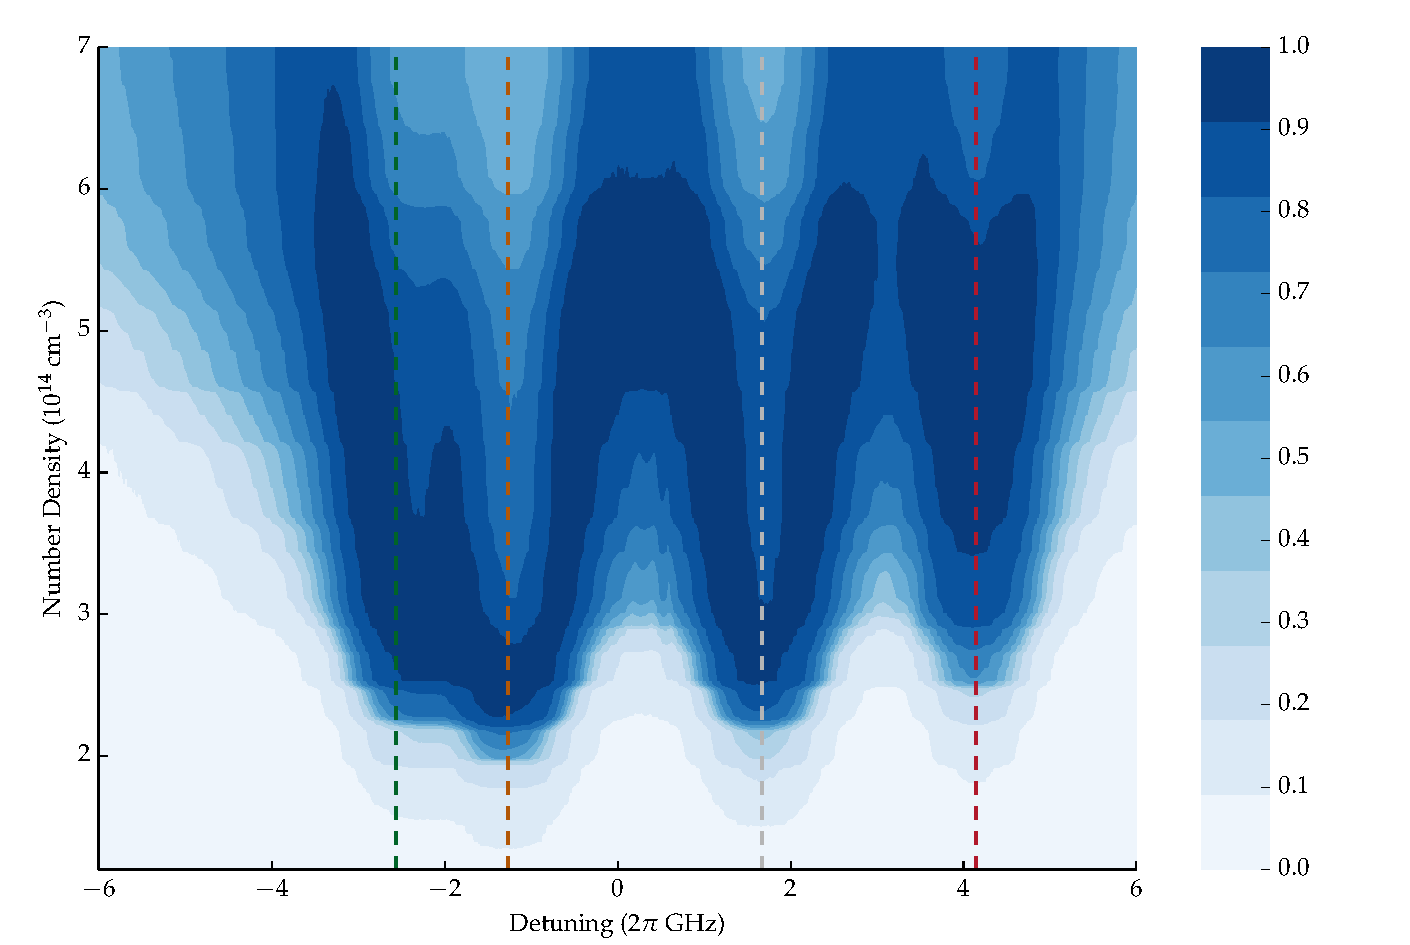
\includegraphics[width=\linewidth]
      {figs/05_twophoton/plot_blue_flourescence_fig1.pdf}
    \caption{
    Normalised experimental fluorescence from the
    $6^2\mathrm{P}_{\nicefrac{1}{2}}$ and $6^2\mathrm{P}_{\nicefrac{3}{2}}$
    transitions, recorded for light input across a GHz detuning range covering
    the \textsc{d2} lines, and over a range of number densities $N$ (and thus
    temperatures $T$). Data source: Weller, 2013\cite{Weller2013}.
    %[TODO: mark on resonances, dotted lines] [make sure
    %resonance visible at lowest densities] [slices in sub figures as per the
    %paper]
    } 
    \label{fig:blue_flourescence} 
    \end{figure}

    In figure \ref{fig:blue_flourescence} the spectral dependence of the
    measured fluorescence is visible as the laser is scanned over a
    \unit[$12$]{GHz} frequency range covering the \textsc{d2} lines, with the
    zero centred on the centre-of-mass transition of the fine structure
    manifolds. The fluorescence is shown normalised as a function of detuning
    (on the horizontal axis) and number density (on the vertical).

    Even from the lowest number densities measured the data shows fluorescence,
    but the striking feature of these results is the sudden and dramatic
    increase in fluorescence at around \unit[$2\times10^{14}$]{cm$^{-3}$} across
    the fluorescence peaks. Our aim in the theoretical work of this chapter is
    determine whether the dependence of the fluorescence on the number density
    can be understood with a description based on the response of individual
    atoms, or if we must consider collective effects like energy
    pooling\cite{Bearman1978,Hill1979,Namiotka1997}, where inelastic collisions
    between excited atoms results in transfer to states with higher energies, or
    cooperative effects arriving from dipole-dipole
    interactions\cite{Keaveney2012a,Weller2011}.
